
\begin{figure}
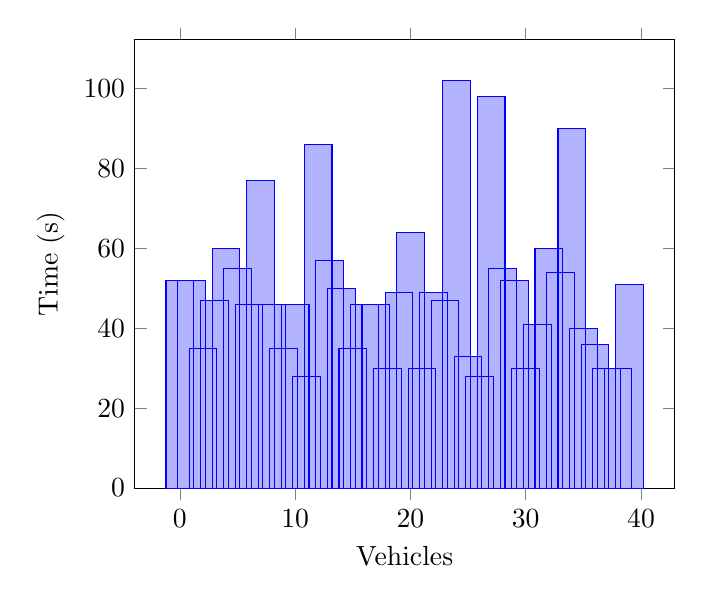
\begin{tikzpicture}
\begin{axis}[
legend style={anchor=west},
xlabel=Vehicles,
ylabel=Time (s),
ymin=0,
ybar,
]
\addplot coordinates {
(0, 52)
(1, 52)
(2, 35)
(3, 47)
(4, 60)
(5, 55)
(6, 46)
(7, 77)
(8, 46)
(9, 35)
(10, 46)
(11, 28)
(12, 86)
(13, 57)
(14, 50)
(15, 35)
(16, 46)
(17, 46)
(18, 30)
(19, 49)
(20, 64)
(21, 30)
(22, 49)
(23, 47)
(24, 102)
(25, 33)
(26, 28)
(27, 98)
(28, 55)
(29, 52)
(30, 30)
(31, 41)
(32, 60)
(33, 54)
(34, 90)
(35, 40)
(36, 36)
(37, 30)
(38, 30)
(39, 51)
};

\end{axis}
\end{tikzpicture}
\label{tik:100:18_N, 18_N.-60, 19_V}
\caption{100 percent diving with GSC on route $18_N, 18_N.-60, 19_V$}
\end{figure}
